\chapter{Litterature}


\section{Images}





\section{Edge detection}

Edge detection regroups differents mathematical methods, where the goal is to identify the change of brightness in the images. An edge is defined as the segments points in where the brightness changes \cite{bib:filter:wikipedia}. Three edge detection methods will be presented in this section : the Sobel, the Laplacian and the Canny operators. These operations detect edges by applying a convolution between an image and a certain mask. The differents masks are given in the \vref{tab:edge detection:masks}.

\begin{table}[ht]	
	\begin{subtable}[b]{0.2\textwidth}
		\centering
		\begin{tabular}{|c|c|c|}
			\hline 
			-1 & 0 & 1 \\ \hline
			-2 & 0 & 2 \\ \hline
			-1 & 0 & 1 \\ \hline
		\end{tabular}
		\caption{Sobel, X axis}
		\label{tab:edge detection:sobel:x}
	\end{subtable}% 
	\begin{subtable}[b]{0.2\textwidth}
		\centering
		\begin{tabular}{|c|c|c|}
			\hline 
			-1 & -2 & -1 \\ \hline
			0 & 0 & 0 \\ \hline
			1 & 2 & 1 \\ \hline
		\end{tabular}
		\caption{Sobel, Y axis}
		\label{tab:edge detection:sobel:y}	
	\end{subtable}%
	\begin{subtable}[b]{0.2\textwidth}
		\centering
		\begin{tabular}{|c|c|c|}
			\hline 
			-1 & -1 & -1 \\ \hline
			-1 & 8  & 0 \\ \hline
			-1 & -1 & -1 \\ \hline
		\end{tabular}
		\caption{Laplacian filter}
		\label{tab:edge detection:laplacian}
	\end{subtable}% 
	\begin{subtable}[b]{0.2\textwidth}
		\centering
		\begin{tabular}{|c|c|c|}
			\hline
			-1 & 0 & 1 \\ \hline
		\end{tabular}
		\caption{Canny, X axis}
		\label{tab:edge detection:canny:x}
	\end{subtable}%
	\begin{subtable}[b]{0.2\textwidth}
		\centering
		\begin{tabular}{|c|}
			\hline
			-1 \\ \hline
			0 \\ \hline
			1 \\ \hline
		\end{tabular}
		\caption{Canny, Y axis}
		\label{tab:edge detection:canny:y}
	\end{subtable}
	
	\centering 
	\caption{Edge detection masks}
	\label{tab:edge detection:masks}
\end{table}

% présentation des 3 filtres 

%The Sobel operator can be obtain by using a convolution between each pixel of the images and the 


The Sobel operator calculates the gradiant of each pixel on the image. It is done by applying a convolution on the image with the two masks given on \vref{tab:edge detection:sobel:x,tab:edge detection:sobel:y}, which are filters that estimates the gradiant in the horizontal and vertical direction  \cite{bib:filter:sobelRuby}. $G_x$ will be the result of the convolution between the image and the $x$ axis filter (same for $G_y$ but with the $y$ axis filter). The gradiant of the resulting image can then be obtain by applying the \vref{eq:edge detection:gradiant}. The Canny operator works in the same way as the Sobel operator. Moreover, the \vref{eq:edge detection:gradiant} can be simplified as the \vref{eq:edge detection:gradiant:simplified} using the manhattan distance \cite{bib:filter:canny}. The first equation will be used for sobel, and the second for canny. 

% The gradient of the image is calculated for each pixel position in the image. 

\noindent\begin{tabularx}{\textwidth}{@{}XX@{}}
	\begin{equation} \label{eq:edge detection:gradiant}
		|G| = \sqrt{G_{x}^2 + G_{y}^2}
	\end{equation} & 
	\begin{equation} \label{eq:edge detection:gradiant:simplified}
		G = |G_x| + |G_y|
	\end{equation}
\end{tabularx}


% simplifié quelque fois avec la distance de manhatan -> G + ABS GX + ABS GY 
% 


\section{Noise removal}




\subsection{Cellular Automata algorithm}

The algorithms presented in the paper \cite{bib:filter:CA} are image noise reduction algorithms based on cellular automata. For this project, it has been decided to implement the second version of the algorithm. A cellular automaton concists of a large number of simple individuals, called cells, which have a state (e.g. "on" and "off"). During one iteration, each cell updates its state depending on its own state and on the state of the neighbor cells. Two types od neighborhooh exists : the 4-connexity (Von Neumann) and the 8-connexity (Moore) neighborhood. For this algorithm, it is the Moor neighborhood that is used. In the case of the second algorithm, each pixel will be updated by taking the average value of his 8-connexity neighborhood (him included), except the minimum and the maximum values. The \vref{fig:diagram:flowchart:CAII} explains the procedure with a flowchart.


%\begin{wrapfigure}{R}{0.4\textwidth}
\begin{figure}[ht]
	\centering
	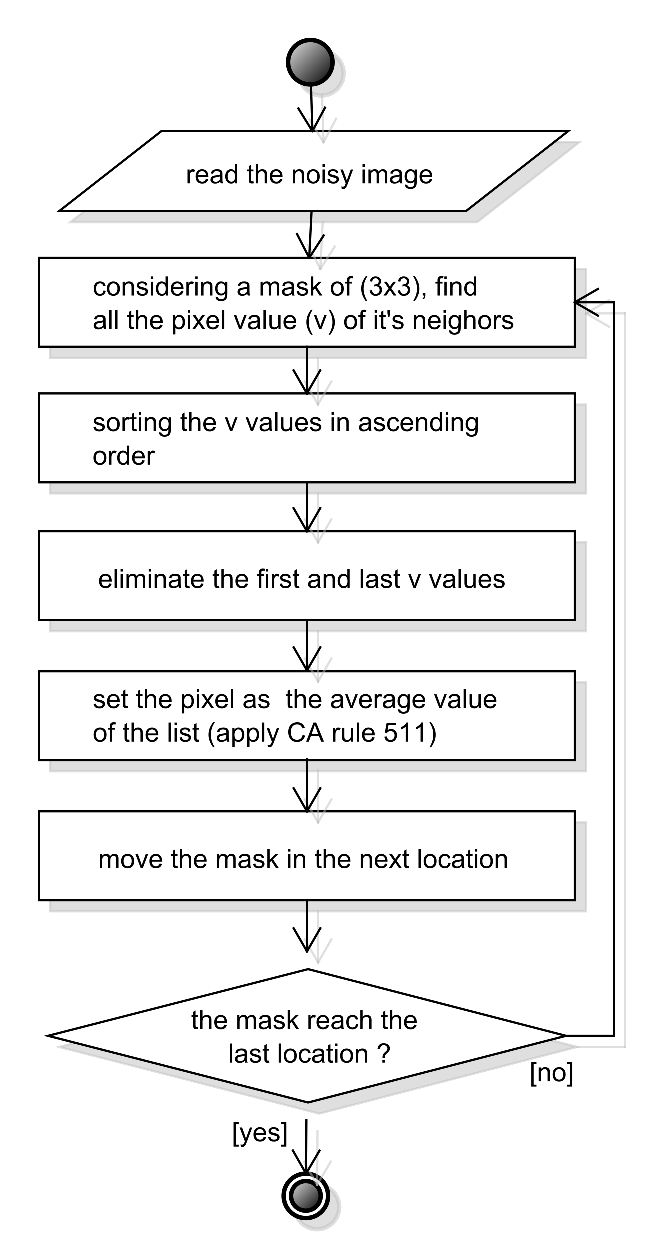
\includegraphics[width=0.4\textwidth]{images/diagrams/flowchart_CAII}
	\caption{CA II flowchart \cite{bib:filter:CA}}
	\label{fig:diagram:flowchart:CAII}
\end{figure}
%\end{wrapfigure}







\section{CLAP}



\section{La dernière....}
